\usepackage{tikz}
\section{Demostración de NP-Completitud}

Para demostrar que la versión de decisión del problema de \textit{Hitting-Set} es NP-Completo, debemos satisfacer dos condiciones:
\begin{enumerate}
    \item Demostrar que pertenece a la clase NP (demostrado en la sección anterior).
    \item Demostrar que un problema NP-Completo conocido se puede reducir en tiempo polinomial a \textit{Hitting-Set}.
\end{enumerate}

Para este segundo paso, elegimos reducir desde el problema de \textbf{Dominating Set} (Conjunto Dominante), el cual se sabe que es NP-Completo.

\subsection{Transformación (Reducción Polinomial)}

Dada una instancia genérica de \textit{Dominating Set} compuesta por un grafo no dirigido $G = (V, E)$ y un entero $k$, construiremos una instancia equivalente para \textit{Hitting-Set} de la siguiente manera:

\begin{itemize}
    \item \textbf{Universo $A$:} Definimos el conjunto universal de elementos como los vértices del grafo. Es decir, $A = V$.
    \item \textbf{Subconjuntos $B_i$:} Para cada vértice $v \in V$, creamos exactamente un subconjunto $B_v$. Los elementos de $B_v$ serán el propio vértice $v$ y todos sus vecinos directos en el grafo. Matemáticamente, esto se corresponde con la vecindad cerrada de $v$: $B_v = N[v]$.
    \item \textbf{Parámetro $k$:} Mantenemos el mismo límite de tamaño $k$.
\end{itemize}

Esta construcción recorre cada vértice y sus aristas adyacentes para armar los conjuntos. Por lo tanto, su complejidad temporal está acotada por $\mathcal{O}(|V| + |E|)$, lo cual garantiza que la transformación se realiza en \textbf{tiempo polinomial}.

\subsection{Ejemplo Gráfico de la Reducción}

Para ilustrar la transformación, utilizaremos un grafo de ejemplo arbitrario (ver Figura \ref{fig:grafo_ejemplo}) con 8 vértices ($a, b, c, d, e, f, g, h$). Este grafo presenta un nodo central y un componente aislado, lo cual es ideal para visualizar la construcción de los subconjuntos.

\begin{figure}[htbp]
    \centering
    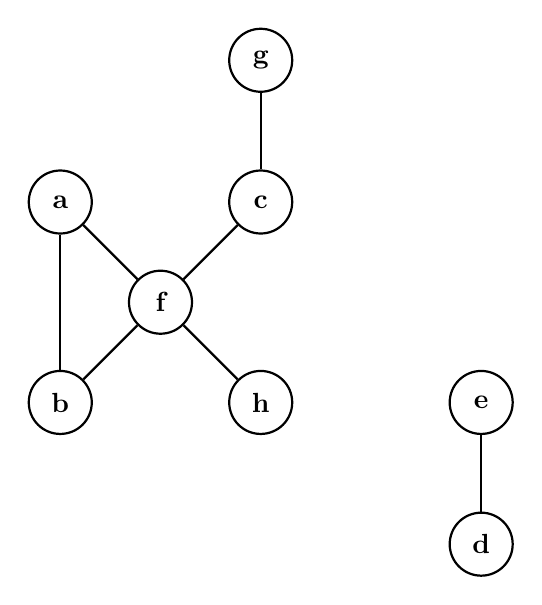
\begin{tikzpicture}[
        node distance=1.8cm,
        nodo/.style={circle, draw=black, thick, minimum size=8mm, font=\bfseries}
    ]
        % Nodos del grafo
        \node[nodo] (f) {f};
        \node[nodo] (a) [above left of=f] {a};
        \node[nodo] (b) [below left of=f] {b};
        \node[nodo] (c) [above right of=f] {c};
        \node[nodo] (h) [below right of=f] {h};
        \node[nodo] (g) [above of=c] {g};
        
        \node[nodo] (e) [right of=h, xshift=1cm] {e};
        \node[nodo] (d) [below of=e] {d};

        % Aristas
        \draw[thick] (a) -- (b);
        \draw[thick] (a) -- (f);
        \draw[thick] (b) -- (f);
        \draw[thick] (c) -- (f);
        \draw[thick] (g) -- (c);
        \draw[thick] (f) -- (h);
        \draw[thick] (e) -- (d);
    \end{tikzpicture}
    \caption{Grafo original de ejemplo utilizado para instanciar el problema de Dominating Set.}
    \label{fig:grafo_ejemplo}
\end{figure}

Al aplicar nuestra función de reducción polinomial, transformamos este grafo en una instancia de \textit{Hitting-Set} donde el universo es $A = \{a, b, c, d, e, f, g, h\}$. Generamos un subconjunto $B_v$ por cada vértice en base a sus vértices adyacentes ($B_v = N[v]$):

\begin{itemize}
    \item $B_a = \{a, b, f\}$
    \item $B_b = \{b, a, f\}$
    \item $B_c = \{c, g, f\}$
    \item $B_d = \{d, e\}$
    \item $B_e = \{e, d\}$
    \item $B_f = \{a, b, c, f, h\}$
    \item $B_g = \{g, c\}$
    \item $B_h = \{h, f\}$
\end{itemize}

Para visualizar esta nueva instancia, podemos representar los subconjuntos como agrupaciones que encierran a sus respectivos elementos, tal como se observa en la Figura \ref{fig:hitting_set}. 

\begin{figure}[htbp]
    \centering
    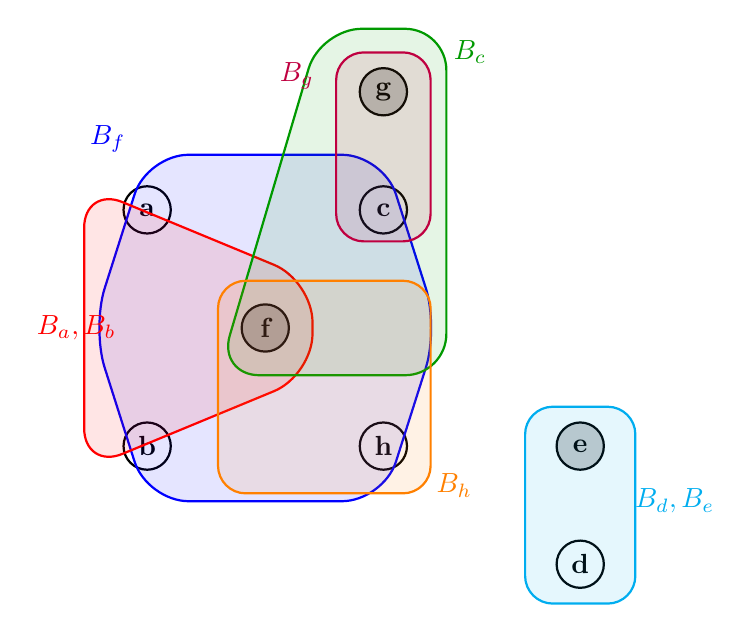
\begin{tikzpicture}[
        nodo/.style={circle, draw=black, thick, minimum size=6mm, inner sep=0pt, font=\bfseries}
    ]
        % Nodos
        \node[nodo, fill=gray!40] (f) at (0,0) {f};
        \node[nodo] (a) at (-1.5, 1.5) {a};
        \node[nodo] (b) at (-1.5, -1.5) {b};
        \node[nodo] (c) at (1.5, 1.5) {c};
        \node[nodo] (h) at (1.5, -1.5) {h};
        \node[nodo, fill=gray!40] (g) at (1.5, 3) {g};
        \node[nodo, fill=gray!40] (e) at (4, -1.5) {e};
        \node[nodo] (d) at (4, -3) {d};

        % Dibujo de los conjuntos
        \begin{scope}[fill opacity=0.1, text opacity=1, thick]
            % Bf
            \draw[fill=blue, draw=blue, rounded corners=15pt] 
                (-2.2, 0) -- (-1.5, 2.2) -- (1.5, 2.2) -- (2.2, 0) -- (1.5, -2.2) -- (-1.5, -2.2) -- cycle;
            \node[blue] at (-2, 2.4) {$B_f$};

            % Ba y Bb
            \draw[fill=red, draw=red, rounded corners=15pt] 
                (-2.3, 1.8) -- (0.6, 0.6) -- (0.6, -0.6) -- (-2.3, -1.8) -- cycle;
            \node[red] at (-2.4, 0) {$B_a, B_b$};

            % Bc
            \draw[fill=green!60!black, draw=green!60!black, rounded corners=15pt] 
                (-0.6, -0.6) -- (2.3, -0.6) -- (2.3, 3.8) -- (0.7, 3.8) -- cycle;
            \node[green!60!black] at (2.6, 3.5) {$B_c$};

            % Bg
            \draw[fill=purple, draw=purple, rounded corners=10pt] 
                (0.9, 1.1) -- (2.1, 1.1) -- (2.1, 3.5) -- (0.9, 3.5) -- cycle;
            \node[purple] at (0.4, 3.2) {$B_g$};

            % Bh
            \draw[fill=orange, draw=orange, rounded corners=10pt] 
                (-0.6, 0.6) -- (2.1, 0.6) -- (2.1, -2.1) -- (-0.6, -2.1) -- cycle;
            \node[orange] at (2.4, -2) {$B_h$};

            % Bd y Be
            \draw[fill=cyan, draw=cyan, rounded corners=10pt] 
                (3.3, -1) -- (4.7, -1) -- (4.7, -3.5) -- (3.3, -3.5) -- cycle;
            \node[cyan] at (5.2, -2.2) {$B_d, B_e$};
        \end{scope}
    \end{tikzpicture}
    \caption{Representación del Hitting-Set. Los globos de colores representan los subconjuntos generados. Los nodos sombreados corresponden a la solución $C = \{f, g, e\}$, demostrando cómo intersecan a la totalidad de los subconjuntos.}
    \label{fig:hitting_set}
\end{figure}

\textbf{Correspondencia de la solución:}
Si resolvemos \textit{Dominating Set} en el grafo original (Figura \ref{fig:grafo_ejemplo}), la solución óptima es $D = \{f, g, e\}$. 
\begin{enumerate}
    \item El nodo \textbf{$f$} domina a $\{a, b, c, f, h\}$.
    \item El nodo \textbf{$g$} domina a $\{g, c\}$.
    \item El nodo \textbf{$e$} domina a $\{e, d\}$.
\end{enumerate}

\subsection{Demostración de Correctitud (Si y solo si)}

Para que la reducción sea válida, debemos demostrar que la instancia original de \textit{Dominating Set} tiene respuesta afirmativa si y solo si la instancia construida de \textit{Hitting-Set} también la tiene.

\subsubsection*{\textit{Si el grafo $G$ tiene un Conjunto Dominante $D$ de tamaño $\leq k$, entonces existe un Hitting-Set $C$ de tamaño $\leq k$ para los subconjuntos construidos.}}


Supongamos que $D$ es un conjunto dominante válido de $G$. Proponemos que nuestro \textit{Hitting-Set} sea exactamente el mismo conjunto de vértices ($C = D$). Debemos probar que $C$ tiene al menos un elemento en común con cada subconjunto $B_v$.

Tomemos un subconjunto cualquiera $B_v$. Por nuestra construcción, $B_v$ contiene al vértice $v$ y a todos sus vecinos. Como $D$ es un conjunto dominante, sabemos por definición que el vértice $v$ pertenece a $D$, o bien al menos uno de sus vecinos pertenece a $D$. En cualquier caso, al menos un elemento de $D$ (nuestro conjunto $C$) se encuentra en $B_v$.

Por lo tanto, $C \cap B_v \neq \emptyset$ para todo $v \in V$, demostrando que $C$ es un \textit{Hitting-Set} válido de tamaño $\leq k$.

\subsubsection*{\textit{Si existe un Hitting-Set $C$ de tamaño $\leq k$ para los subconjuntos construidos, entonces el grafo $G$ original tiene un Conjunto Dominante $D$ de tamaño $\leq k$.}}


Supongamos que existe un \textit{Hitting-Set} $C$ válido de tamaño $\leq k$. Proponemos que nuestro Conjunto Dominante sea exactamente ese conjunto ($D = C$). Debemos probar que todo vértice $v \in V$ está dominado por $D$.

Tomemos un vértice cualquiera $v \in V$. En nuestra instancia de \textit{Hitting-Set}, existe un subconjunto $B_v$ que representa la vecindad cerrada de dicho vértice. Como $C$ es un \textit{Hitting-Set}, sabemos que obligatoriamente intersecta a $B_v$, lo que implica que existe un elemento $u \in C$ tal que $u \in B_v$.

Dado que los únicos elementos dentro de $B_v$ son el propio $v$ y sus vecinos, esto significa que el vértice $u$ (que pertenece a $D$) es el propio vértice $v$ o es adyacente a él. En ambos escenarios, el vértice $v$ resulta dominado por un elemento de $D$.

Como esto se cumple para todo vértice en $V$, $D$ es un Conjunto Dominante válido de tamaño $\leq k$.

\vspace{0.5cm}
\textbf{Conclusión:} Al haber demostrado la pertenencia a NP y haber establecido una reducción polinomial válida desde un problema NP-Completo (\textit{Dominating Set}), se concluye formalmente que el problema de decisión de \textit{Hitting-Set} es \textbf{NP-Completo}.